\documentclass[11pt, a4paper]{report}
\usepackage{graphicx}
\usepackage[table,xcdraw]{xcolor}
\usepackage{geometry}
\usepackage{float}
\usepackage{authblk}
\usepackage{anyfontsize}
\usepackage[document]{ragged2e}
\usepackage{titlesec}
\usepackage[parfill]{parskip}
\usepackage{color}   %May be necessary if you want to color links
\usepackage{hyperref}
\usepackage{caption}
\usepackage{tabularx}
\usepackage{longtable}
\usepackage{blindtext}
\hypersetup{
    colorlinks=true, %set true if you want colored links
    linktoc=all,     %set to all if you want both sections and subsections linked
    linkcolor=black,  %choose some color if you want links to stand out
}
\titleformat{\chapter}[hang] 
{\normalfont\huge\bfseries}{\chaptertitlename\ \thechapter:}{1em}{} 
\geometry{left=2.5cm,right=2.5cm,top=2.5cm,bottom=2.5cm}
\graphicspath{ {./images/} }

\begin{document}  
    \pagestyle{empty}
\centering
\fontsize{2cm}{2cm}\selectfont{Module Design Document} \\
\vspace{2mm}
\fontsize{1cm}{1cm}\selectfont Audio digital signal processor \\
\vspace{2mm}
\large BeCreative Minor\\
\normalsize
\vspace{4cm}
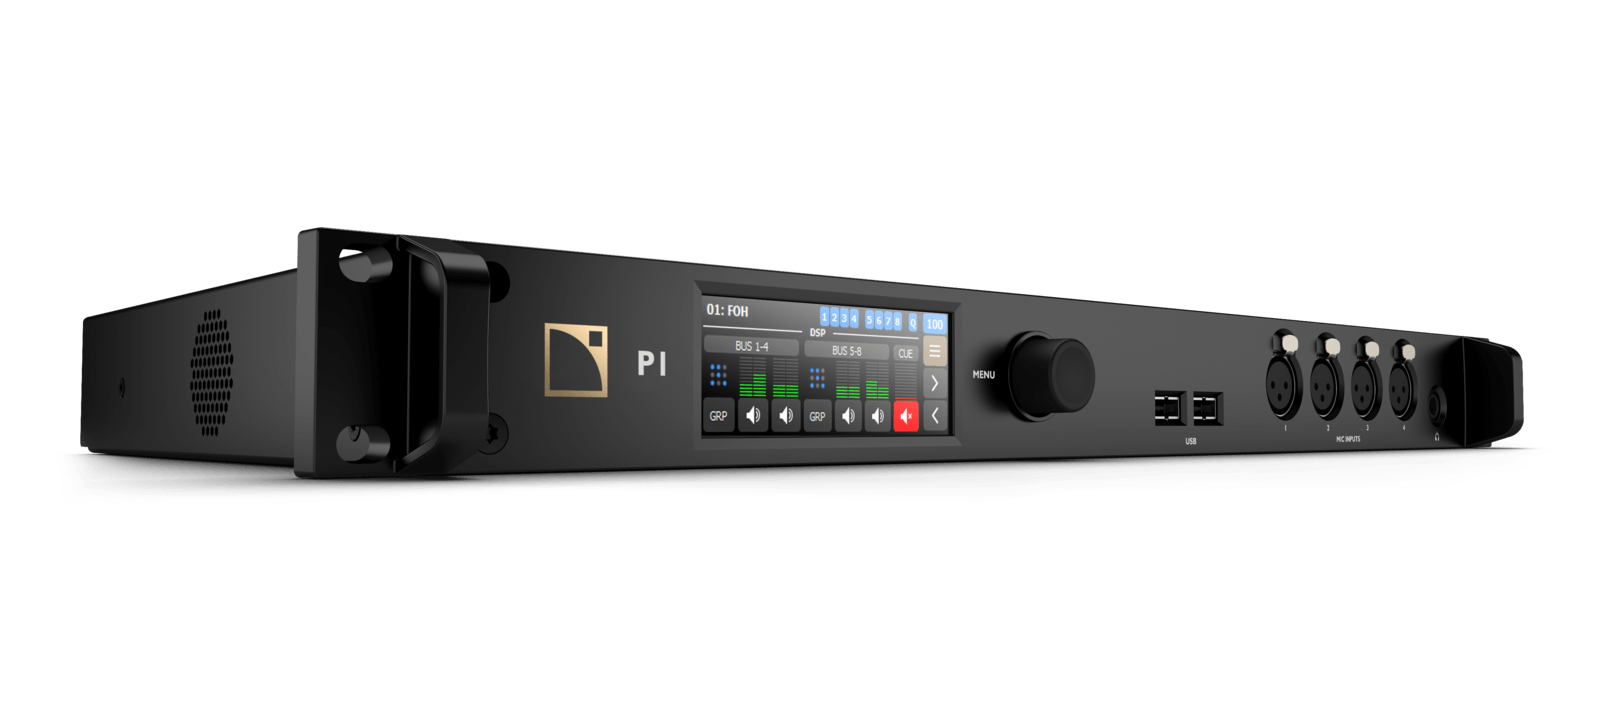
\includegraphics[width=\linewidth]{3DR_P1_Perspective.png}\\
\vfill
\normalsize Busse Lommers \\
Robin van den Dungen \\
Mahmud Gürler \\
Silas Kamphuis \\
Hein Verhallen \\
Youri Tils \\
Fontys Hogescholen, De Rondom 1, 5612 AP Eindhoven \\
\today

\begin{justify}

\chapter*{Summary}
The following text translates to English as:

This report describes how this project group created an audio DSP for the BeCreative Minor. This was done because the members of the group wanted to learn more about it and improve their technical knowledge.

Chapter "Problem Description" outlines the project's background and goals. Chapter "Research" describes the preliminary investigations conducted. Chapter "Concept Development" explains how the product concept was developed. Chapter "Realization" details the actual design of the audio DSP. Chapter "Verification" discusses the product testing process. Finally, in chapters "Conclusions" and "Recommendations," the conclusion and recommendations are respectively described.

\newpage
\tableofcontents
\thispagestyle{empty}

\listoffigures
\thispagestyle{empty}

\listoftables
\thispagestyle{empty}

\newpage
\pagestyle{plain}

\chapter*{Report contribution}	%Fill-in only regarding the report contribution.
\begin{longtable}{|c|c|c|}
	\hline
	\textbf{Chapter} & \textbf{Paragraph} & \textbf{Person} \\ \hline
	Problem Description			& Background					& All	 					\\ \hline
	Introduction				& NA							& Busse 					\\ \hline
								& Problem description			& Robin						\\ \hline
								& Project goals					& All						\\ \hline
								& Requirements					& All 						\\ \hline
								& Project scope					& All 						\\ \hline
								& Boundary condition			& All						\\ \hline
								& Project approach				& All						\\ \hline
								& Verification method			& All						\\ \hline
	Research 					& Research objectives			& All 						\\ \hline
								& Research questions			& All 						\\ \hline
								& Research approach				& All 						\\ \hline
								& Results						& All 						\\ \hline
	Concept Development 		& Concept overview				& Youri						\\ \hline
								& Front-end						& Silas						\\ \hline
								& Audio-DSP						& Youri						\\ \hline
								& Back-end						& Silas						\\ \hline
								& Interfacing					& Robin						\\ \hline
								& Front-end						& Robin						\\ \hline
								& Audio-DSP						& Youri						\\ \hline
								& Back-end						& Robin						\\ \hline
								& Power supplies				& Mahmud \& Robin			\\ \hline
								& Modules						& Busse						\\ \hline
								& UI							& Hein \& Busse				\\ \hline
								& Hardware programming			& Busse						\\ \hline
								& Hardware design				& Busse						\\ \hline
								& Design decissions				& Busse						\\ \hline
	Realization					& Hardware						& NA						\\ \hline
								& Schematic						& Robin						\\ \hline
								& Printed circuit board			& Silas						\\ \hline
								& Case							& Busse						\\ \hline
								& Firmware						& Youri						\\ \hline
								& I2S decoder and encoder		& Youri						\\ \hline
								& I2C controller				& Youri						\\ \hline
								& Band-pass filter				& Youri						\\ \hline
								& Sinewave generator			& Youri						\\ \hline
								& Effects						& Youri \& Busse			\\ \hline
								& User interface				& Hein \& Busse				\\ \hline
								& User interface				& Hein \& Busse				\\ \hline
	Verification				& Method						& Robin						\\ \hline
								& Hardware						& Mahmud \& Robin			\\ \hline
								& Firmware						& Youri						\\ \hline
								& Results						& NA						\\ \hline
								& Hardware						& Mahmud					\\ \hline
								& Firmware						& Youri						\\ \hline
								& Conclusions					& Mahmud \& Silas \& Robin 	\\ \hline
								& Hardware						& Mahmud					\\ \hline
								& Firmware						& Youri						\\ \hline
	Conclusions					& NA							& Silas						\\ \hline
	Recommendations				& NA							& Silas						\\ \hline
	Summary						& NA							& Robin						\\ \hline
	Bibliography				& NA							& Busse						\\ \hline
	Appendix A: State-space		& NA							& Youri						\\ \hline
	Appendix B: VHDL code		& I2S decoder					& Youri						\\ \hline
								& I2S encoder					& Youri						\\ \hline
								& I2C master					& Youri						\\ \hline
								& State-space BPF code			& Youri						\\ \hline
								& Sinewave generator code		& Youri						\\ \hline
	Appendix C: Schematics		& Buck converter schematic		& Mahmud					\\ \hline
								& SEPIC schematic				& Silas						\\ \hline
								& Linear regulator schematic	& Silas	\& Robin			\\ \hline
								& Main board schematic			& Robin						\\ \hline
								& Buck converter calculations	& Silas						\\ \hline
								& SEPIC calculations			& Robin						\\ \hline
	Appendix D: UI design		& Main menu						& Busse						\\ \hline
								& Adjust preset menu			& Busse						\\ \hline
	Appendix E: Case			& Top view						& Busse						\\ \hline
								& Front view					& Busse						\\ \hline
								& Rear view						& Busse						\\ \hline
	Appendix F: Verification	& Ground spring					& Robin						\\ \hline

	\caption{Revision list of the document}
	\label{table:revision_history}
\end{longtable}

\newpage
\pagestyle{plain}
\setcounter{page}{1}

\chapter*{Abbreviation List}

\begin{table}[!h]
	\centering
	\begin{tabular}{|c|c|}
		\hline
		\textbf{Abbreviation} & \textbf{Explanation}	\\ \hline
		DSP 					& Digital Signal Processor    				\\ \hline
		ADC 					& Analog-to-Digital Converter 				\\ \hline
		BPF 					& Band-Pass Filter							\\ \hline
		CH 						& Channel									\\ \hline
		DAC 					& Digital-to-Analog Converter 				\\ \hline
		FFT 					& Fast Fourier Transform					\\ \hline
		FPGA 					& Field programmable gate array 			\\ \hline
		GBW 					& Gain Bandwidth Product 					\\ \hline
		RAM 					& Random Access Memory	    				\\ \hline
		SEPIC        			& Single-Ended Primary-Inductor Converter	\\ \hline
		SINAD 					& Signal to noise and distortion 			\\ \hline
		TRS 					& Tip ring sleeve connector (jack) 			\\ \hline
	\end{tabular}
	\caption{List of commonly used Abbreviations}
	\label{table:Abbreviation list}
\end{table}

    \chapter{Background}
        %BACKGROUND
When listening to music it is of great importance that the speakers are tuned to the environment and the position of the listener. This is necessary to achieve the best experience. If the speakers are not correctly tuned to the surrounding environment, a digital signal processor (DSP) is used to correct this. A DSP is a specialized processor which is used for digital signal processing. 

In the audio world a DSP is used to optimize a sound system. For example some speakers have some imperfections and a DSP can be used to correct for these imperfections. It is also often used to add more dynamics to sound.


    \chapter{Requirements}
        The goal of this project is to research how to make an audio-DSP. 
This raises the main research question: \textbf{“How to design an audio-DSP?”}. 
In the process of researching this an actual audio-DSP will be developed. 
From the main research question the following sub-research questions are derived:

\begin{itemize}
	\setlength\itemsep{-0.3em}
	\item What is the best method for creating digital filters?
	\item What is the best method for creating digital effects?
	\item What is the most suitable anti-aliasing filter?
	\item What is the optimal needed roll-off for the anti-aliasing filter for a given bandwidth such that the noise can be negligible?
	\item What is the minimum sample frequency needed to capture the desired frequency spectrum?
	\item What is the minimum frequency range to be sampled to achieve sufficient detailed audio?
	\item What is the lowest allowable noise for decent audio?
	\item What ADC resolution is needed such that the quantization error and noise level are on par?
	\item What ADC and DAC architecture is most suitable for this application?
	\item What kind of processor is most suitable for this application?
	\item What is the permittable jitter for accurate audio?
	\item What is the maximum allowable ripple on the reference voltage for the ADC and DAC?
	\item How much RAM does the system need?
	\item How much flash does the system need?
	\item What power supply topology is best suited for each part of the system?
	\item How do we ensure that the USB input of the processor is recognized by Windows as an audio device?
\end{itemize}

\noindent The project is conducted during the minor BeCreative at Fontys. 
This minor takes 20 weeks and allows the students to have a budget of €300,-. 
Thus after 20 weeks starting from 6-2-2023 an audio-DSP will be delivered within a budget of €300,-.

The audio system has some requirements to specify the final result. 
These requirements are derived with the “MoSCoW” method. 
The following requirements are confirmed by the research document.

\newpage
\begin{longtable}{|l|p{10cm}|l|l|}
	\hline
	\textbf{ID} & \textbf{Requirement} & \textbf{Priority} & \textbf{Status}\\ \hline 
	\textbf{U1} & \textbf{Inputs:} \newline
	•Two RCA audio inputs which work on a line level of 4dBu(±1,74V)\newline
	•Two 6,35mm TRS plug audio inputs which work on a line level of 4dBu(±1,74)\newline
	•Two XLR audio which work on a line level of 22dBu(±9,75) 																	& Must	 & Proposed\\ \hline
	\textbf{U2} & \textbf{Outputs:} \newline
	•Two RCA audio outputs which work on a line level of 4dBu(±1,74V)\newline
	•Two 6,35mm TRS plug audio outputs which work on a line level of 4dBu(±1,74V)\newline
	•Two XLR signal outputs which work on a line level of 22dBu(±9,75)															& Must 	 & Proposed\\ \hline
	\textbf{U3} &The system should have a bandwidth (±3 dB) of at least 20 Hz up and till 20 kHz without any filters applied. 	& Must   & Proposed\\ \hline
	\textbf{U4} &The system has an Audio sample rate of at least 192 kHz 														& Must   & Proposed\\ \hline
	\textbf{U5} &The ADC and DAC resolution is at least 16-bit 																	& Must   & Proposed\\ \hline
	\textbf{U6} &Signal-to-noise and distortion (SINAD) is at least 100dB  														& Must   & Proposed\\ \hline
	\textbf{U7} &Anti-aliasing filter is a 6th order filter										 								& Must   & Proposed\\ \hline
	\textbf{U8} &propagation delay of less than 100ms without any filters applied												& Must   & Proposed\\ \hline
	\textbf{U9} &The system has two samplers											 										& Must   & Proposed\\ \hline
	\textbf{U10}&The system has two input channels 																				& Must   & Proposed\\ \hline
	\textbf{U11}&The system has two output channels														 						& Must   & Proposed\\ \hline
	\textbf{U12}&The system has two signal processors														 					& Must   & Proposed\\ \hline
	\textbf{U13}&User can select what input will be routed to what output channel via a user interface							& Must   & Proposed\\ \hline
	\textbf{U14}&All inputs use at least 80\% of the ADC resolution at their specified line level								& Must   & Proposed\\ \hline
	\textbf{U15}&User can select 1 effect to be active in one channel at the same time											& Must   & Proposed\\ \hline
	\textbf{U16}&The 6,35mm TRS plug audio inputs must have a variable gain														& Must   & Proposed\\ \hline
	\textbf{U17}&User can configure each effect															 						& Must   & Proposed\\ \hline
	\textbf{U18}&The system works standalone																					& Must   & Proposed\\ \hline
	\textbf{U19}&The user can configure each effect in the user interface														& Must   & Proposed\\ \hline
	\textbf{U20}&The system has a visual representation of the user interface													& Must   & Proposed\\ \hline
	\textbf{U21}&Effects configurable in each signal processor channel: \newline
	\begin{itemize}
		\setlength\itemsep{-0.4em}
		\item Distortion
		\item Reverb
		\item Gain
		\item Equalizer
		\item Delay
	\end{itemize}																												& Must 	 & Proposed\\ \hline
	\textbf{U22} &An FPGA is used as processor																 					& Must   & Proposed\\ \hline
	\textbf{U23} &RAM is at least 2MB																		 					& Must   & Proposed\\ \hline
	\textbf{U24} &The system has a bandwidth (±1 dB) of at least 20 Hz up and till 20 kHz without any filters applied 			& Should & Proposed\\ \hline
	\textbf{U25} &The ADC and DAC resolution is at least 24-bit.																& Should & Proposed\\ \hline
	\textbf{U26} &Signal-to-noise and distortion (SINAD) is at least 120dB 														& Should & Proposed\\ \hline
	\textbf{U27} &propagation time delay of less than 10ms without any filters applied 											& Should & Proposed\\ \hline
	\textbf{U28} &The system has four input channels 																			& Should & Proposed\\ \hline
	\textbf{U29} &The system has six output channels 																			& Should & Proposed\\ \hline
	\textbf{U30} &The system has six signal processors 																			& Should & Proposed\\ \hline
	\textbf{U31} &The system has a USB audio input					 															& Should & Proposed\\ \hline
	\textbf{U32} &The system has a USB decoder					 																& Should & Proposed\\ \hline
	\textbf{U33} &Six XLR signal outputs work on a line level of 22 dBu (±9,75 V) 												& Should & Proposed\\ \hline
	\textbf{U34} &The system is able to recover the last saved configuration of the effect and the channel routing after reboot	& Should & Proposed\\ \hline
	\textbf{U35} &The system has equalizer presets e.g. Rock, Classical, Default, effect		 								& Should & Proposed\\ \hline
	\textbf{U36} &The system has different effect presets										 								& Should & Proposed\\ \hline
	\textbf{U37} &The system has default settings for channel routing and presets							 					& Should & Proposed\\ \hline
	\textbf{U38} &User can select up to 4 effects to be active in one channel at the same time. 								& Should & Proposed\\ \hline
	\textbf{U39} &Effects configurable in each signal processor channel:\newline
	\begin{itemize}
		\setlength\itemsep{-0.3em}
		\item Phaser
		\item Tremelo
		\item Flanger
		\item Fuzz
		\item Overdrive
		\item Chorus
		\item Compressor
		\item Wah
		\item Looper
		\item Wow and flutter
		\item Modulator
		\item Echo
		\item Fade in/out
		\item Delay (at least 4 seconds)
	\end{itemize}																												& Should & Proposed\\ \hline
	\textbf{U40} &Local power supplies for different parts of the system 														& Should & Proposed\\ \hline
	\textbf{U41} &A custom PCB is designed for the local power supplies, front-end and back-end of the system					& Should & Proposed\\ \hline
	\textbf{U42} &Signal-to-noise and distortion (SINAD) is at least 140dB 														& Could  & Proposed\\ \hline
	\textbf{U43} &The user can configure custom presets for the equalizer, effect and channel routing via the user interface	& Could  & Proposed\\ \hline
	\textbf{U44} &propagation time delay of less than 100µs without any filters applied. 										& Could  & Proposed\\ \hline
	\textbf{U45} &User can select up to 10 effects to be active in one channel at the same time 								& Could  & Proposed\\ \hline
	\textbf{U46} &Touch screen user interface 																					& Could  & Proposed\\ \hline
	\textbf{U47} &Zero-crossing detection to make adjusting the filters happen glitch free										& Could  & Proposed\\ \hline
	\textbf{U48} &Self-made mains power supply  																				& Won't  & Proposed\\ \hline
\end{longtable}
    \end{justify}
\end{document}